\documentclass{article}
\usepackage{graphicx}

\begin{document} 
\begin{center}
{\bf \Large  Homework 6} \\
(Due on: May 20, 9:00PM, by e-mail)
\end{center}


\noindent The state of a body falling vertically through the atmosphere is $\underline{\bf \rm x}=[x\ {\dot x}\ \beta]^T$, 
where $x$ is its height above the Earth's surface and $\beta$ its ballistic coefficient. The ballistic coefficient is included as a state because it is not well known,  so it must be estimated. Use EKF for continuous time models and discrete observations.

The state equations are
\begin{eqnarray}
   \frac{d x}{dt} &=& \dot x \\
   \frac{d {\dot x}}{dt} &=& d-g \\
   \frac{d \beta}{dt} &=& \xi(t)
\end{eqnarray}
 where $g=9.8\  [m/s^2]$ is acceleration due to gravity, $\xi(t)$ is the zero-mean white noise of intensity $1000\  [g^2/(m^2 s^6)]$, 
and the drag is given by 
\begin{equation}
  d= \frac{\rho {\dot x}^2}{2 \beta}
\end{equation}
Units are provided in the rectangular brackets, however the problem is defined so that you do not need to worry about them. 

Atmospheric density is 
\begin{equation}
  \rho = \rho_0 e^{- x /c}
\end{equation}
with $\rho_0=1220\  [g/m^3]$ being the density at sea level and $c=10263\  [m]$ a decay constant.

Suppose range measurements are taken every second (T=1\  [s]) as in the figure (see the next page). Thus, 
\begin{equation}
  z_k=\sqrt{r_1^2+(x_k-r_2)^2 }+ v_k
\end{equation}
with $r_1=1000\  [m]$, $r_2=500\ [m]$,  $x_k=x(kT)$ and $v_k \sim N(0,\sigma^2_r)$,  $\sigma_r^2=5\  [m^2]$.\\


\noindent {\bf (a)} Write down the prediction step of EKF; {\bf (b)} Write down the update step of EKF;  {\bf (c)} Assume that at $t=0$, $E\{ x(0)\}=10000[m]$, $var\{ x(0)\}=50[m^2]$,  $E\{{\dot  x}(0)\}=-500[m/s]$, 
 $var\{ {\dot x}(0)\}=200[m^2/s^2]$, $E\{\beta(0)\}=6 \times 10^7 [g/ms^2]$, 
$var(\beta(0))=2 \times 10^{12} [g^2/m^2 s^4]$ and that the measured data are taken every second 
beginning at $t_1=1[s]$, and are given in meters by 
\begin{equation}
z_1,z_2,....z_{10}= 9055, 8560, 7963, 7467, 7000, 6378, 5885, 5400, 4928, 4503
\end{equation}
Plot the $x_m(k)=\sqrt{z_k^2-r_1^2}+r_2$ and the EKF estimates for $x(t)$ on the same 
diagram. On separate diagrams, plot the velocity ($\dot x$) and the ballistic coefficient ($\beta$) estimates. 

\begin{figure}[h]
\begin{center}
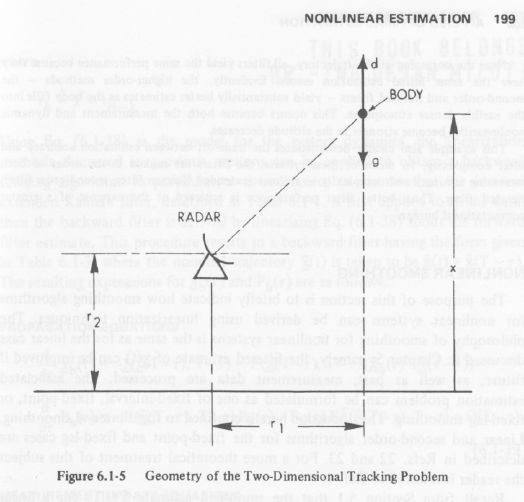
\includegraphics[width=\textwidth]{Radar.png}
\end{center}
\end{figure}

  
\end{document}